\chapter*{Numerical grids}
We distinguish two types of numerical grids: the 3D soil grid and the 1D, branched, root system grid (see Fig. \ref{fig:grids}). 

\begin{figure}[ht]
	\centering
  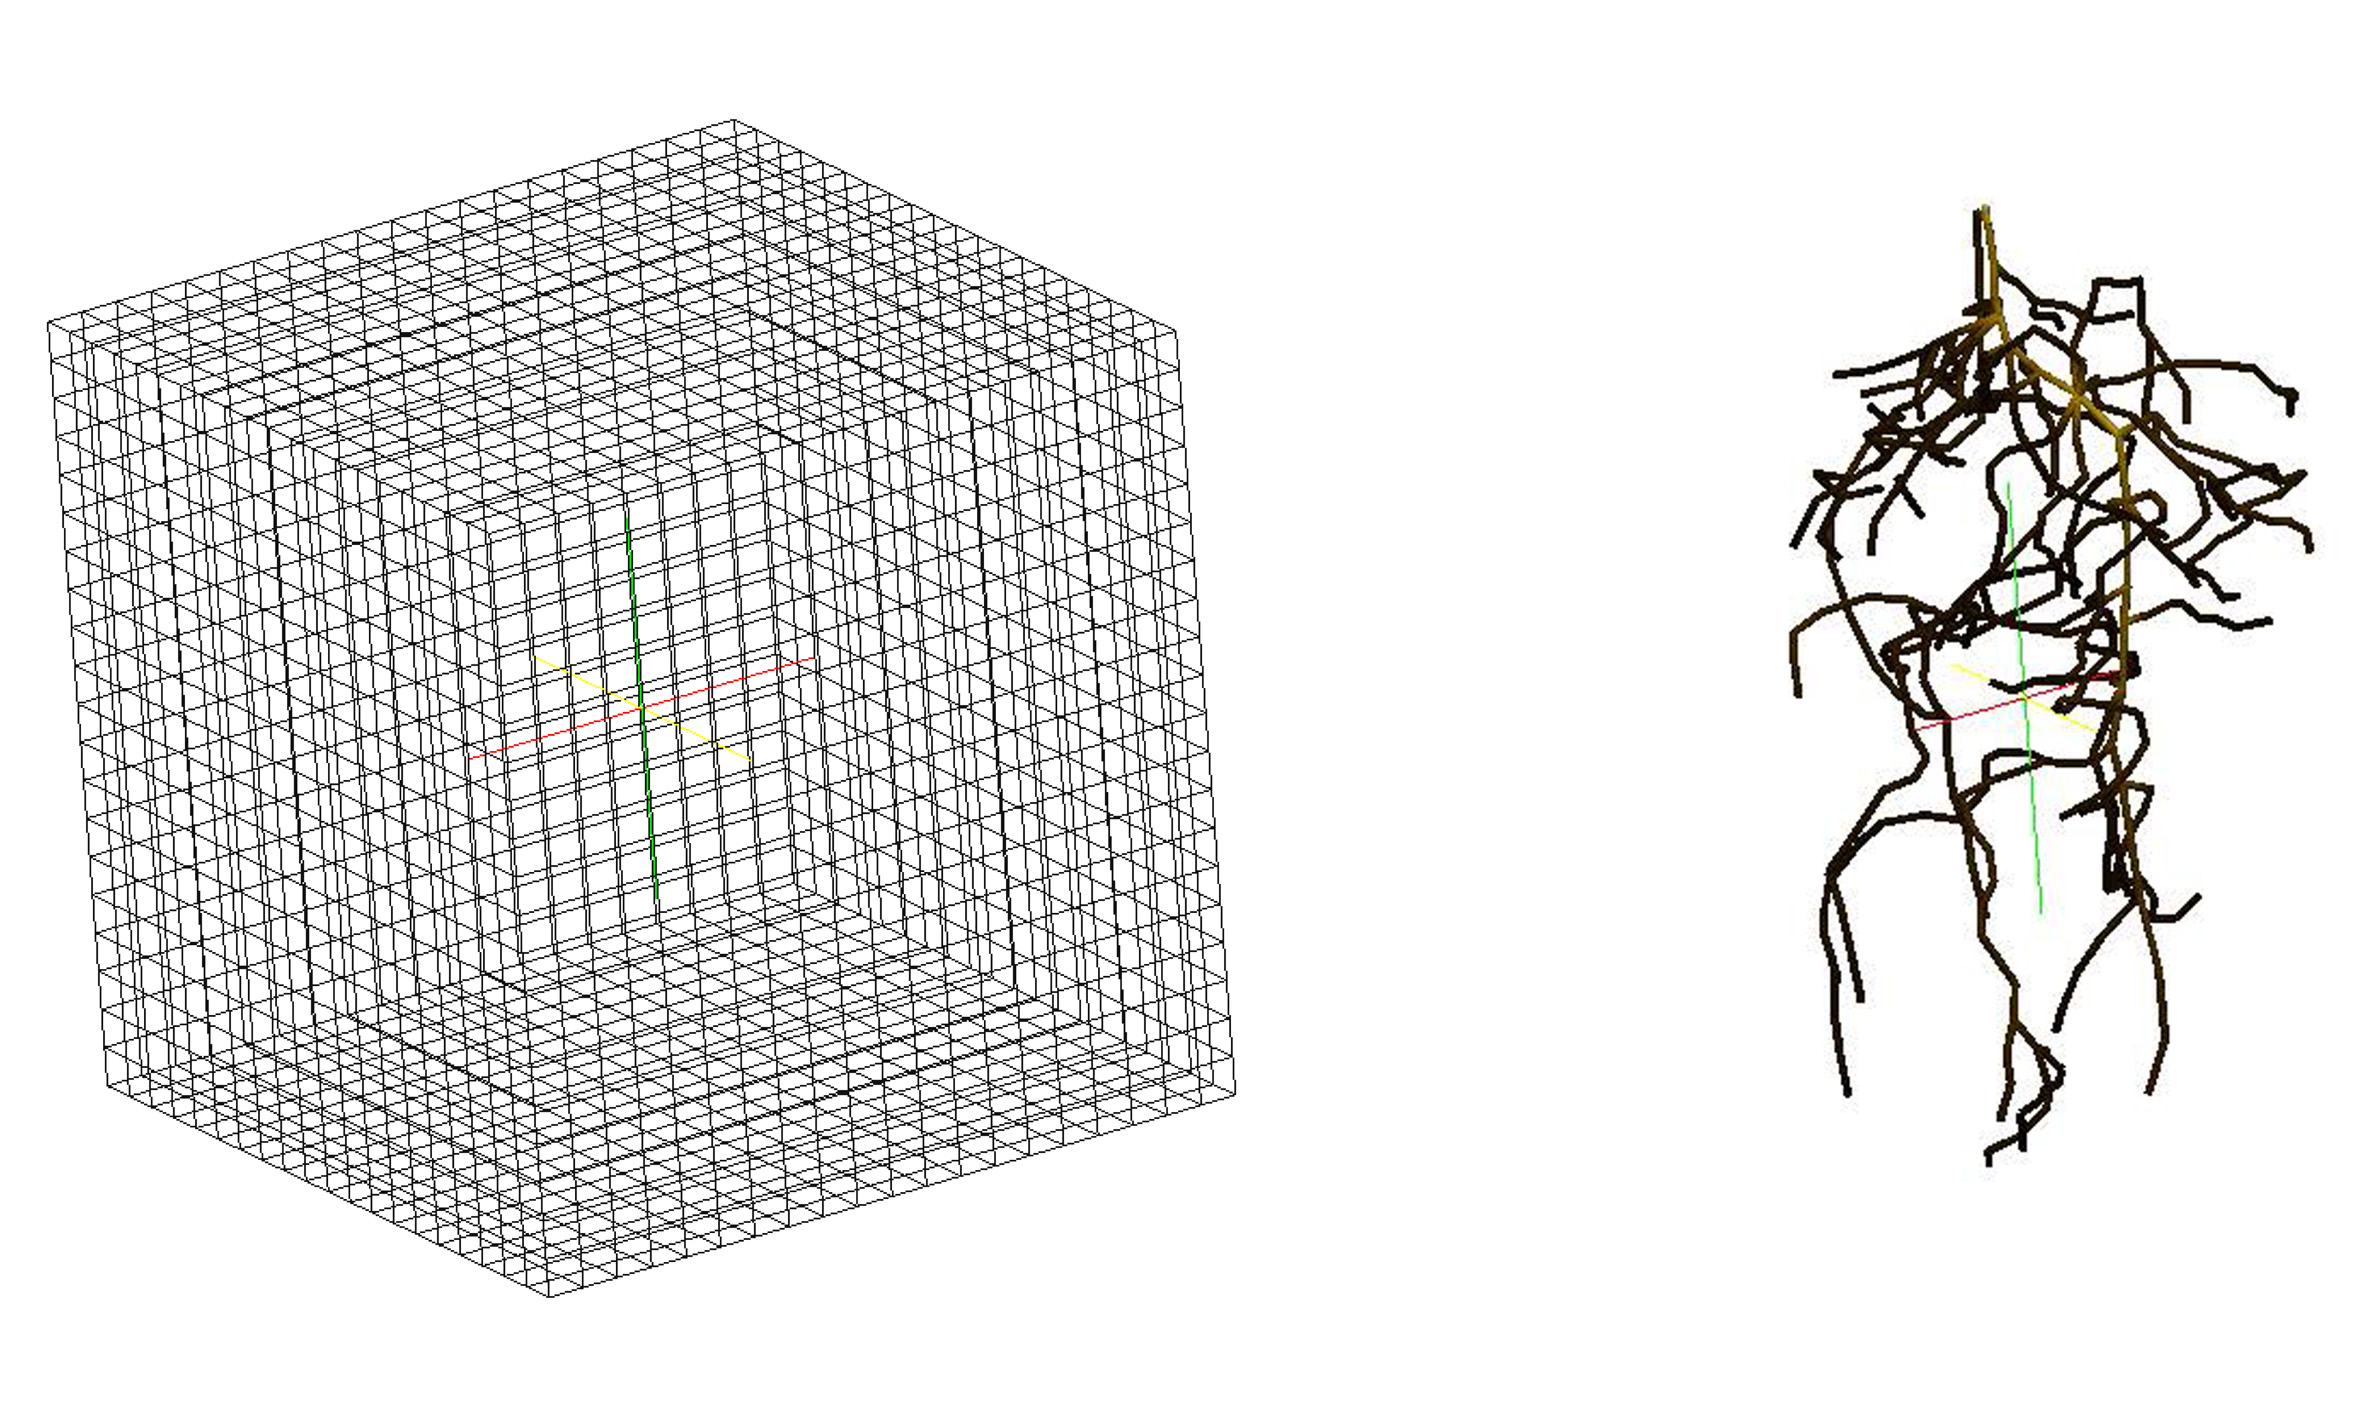
\includegraphics[width=0.5\textwidth]{grids.jpg}
	\caption{The 3D soil grid and the 1D, branched, grid representing the root architecture}
	\label{fig:grids}
\end{figure}

In the example of the coupled problems, both are used simultaneously. In that case, the two grids are merged via source/sink terms in positions where root and soil grids share the same spatial coordinates. This is illustrated in Fig. \ref{fig:merged}; detailed descriptions can be found in the individual examples. 
 
\begin{figure}[ht]
	\centering
  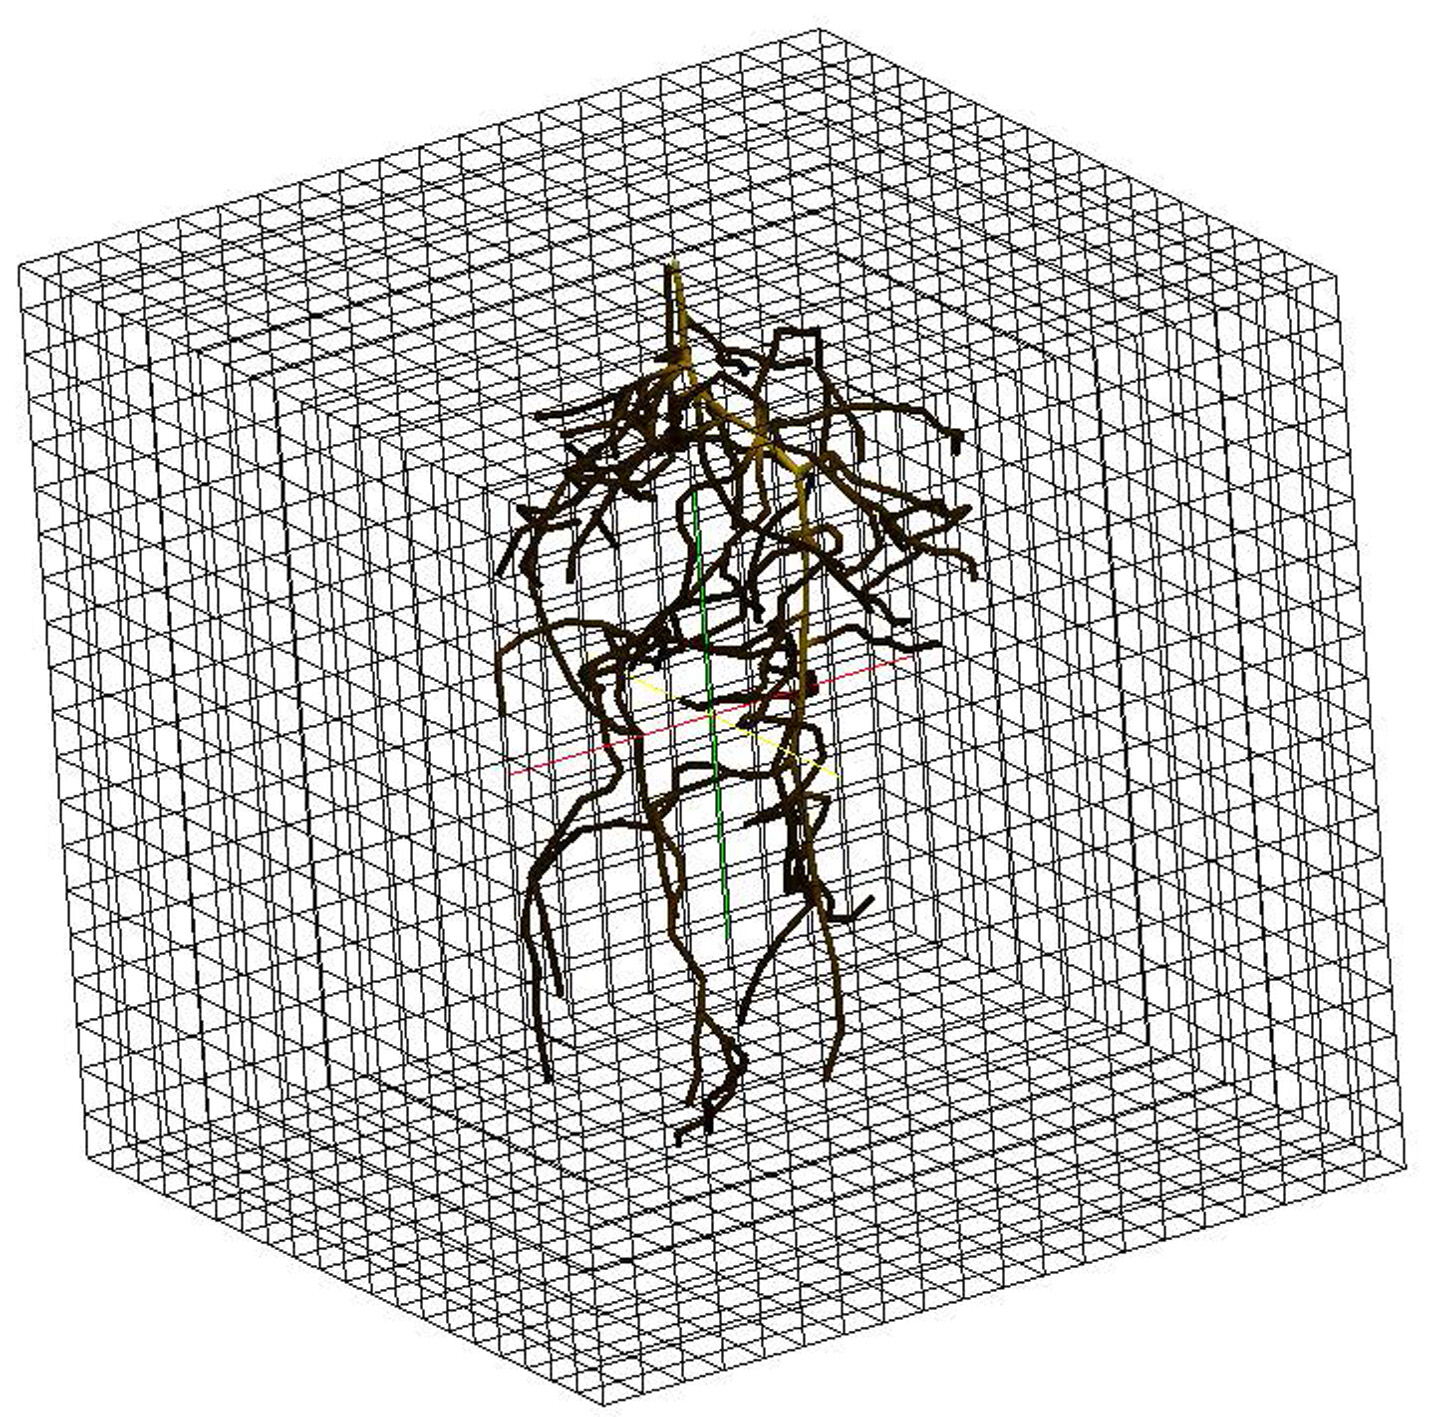
\includegraphics[width=0.33\textwidth]{merged.jpg}
	\caption{3D soil grid merged with the 1D, branched, grid representing the root architecture}
	\label{fig:merged}
\end{figure}

Grids can be created using different DUNE internal or external grid managers (see documentation of dune-grid). In the input file, the details about the numerical grids are specified in the groups [RootSystem.Grid] or [SoilGrid]. Each folder contains a folder named ``grids" where grids can be provided in dgf format. In the dumux-rosi examples, the soil grid is usually a structured grid created by the default ``GridCreator", where corner points of the domain, spatial resolution and cell type are specified such as in the following example: 

\begin{lstlisting}
[ Grid ]
LowerLeft = 0 0 0
UpperRight = 1 1 1
Cells = 10 10 20
CellType = Cube # or Simplex
\end{lstlisting}

There are two options to specify the root system grid. The first option is to specify it as a file in dgf-format that specifies the coordinates and connection of nodes (verteces).  

\begin{lstlisting}
DGF
Vertex
0.050000 0.050000 -0.000000
0.050000 0.050000 -0.0250000
0.050000 0.050000 -0.05000
0.050000 0.050000 -0.075000
#
SIMPLEX 
parameters 10 
0 1 1 0 3.14159e-05 0.01 0.0005 0.00 0.0001 0.00001 21922.1 
1 2 1 0 2.51327e-05 0.008 0.0005 0.00 0.0001 0.00001 39940.5 
2 3 1 0 2.51327e-05 0.008 0.0005 0.00 0.0001 0.00001 58409.5 
3 4 1 0 2.51327e-05 0.008 0.0005 0.00 0.0001 0.00001 77352.1 
4 5 1 0 2.51327e-05 0.008 0.0005 0.00 0.0001 0.00001 96793.2 
5 6 1 0 2.51327e-05 0.008 0.0005 0.00 0.0001 0.00001 116760 
#
BOUNDARYDOMAIN
default 1
#
\end{lstlisting}

The paragraph ``SIMPLEX" specifies 10 parameters for each root segment: node1ID, node2ID, type, branchID, surfaceIdx, length, radiusIdx, massIdx, axialPermIdx, radialPermIdx, creationTimeId in SI units. 

Root systems in dgf format can be computed from measured root systems as well as with the root architecture model CRootBox. 

The second option is to provide the root architectural parameters in the input file such that the root architecture and related grid is computed by CRootBox while used as a DuMu$^x$ module. 

\begin{lstlisting}
[RootSystem.Grid]
File = Triticum_aestivum_a_Bingham_2011  
InitialT = 10 # days
\end{lstlisting}

Important to know: It is currently necessary to build the code either for option 1 or for option 2 (i.e., two executables can be built that need to be provided with the correct input at runtime). 